\chapter{\label{chap:problem}O Problema}
A prática de estabelecer a complexidade computacional de jogos -- sejam jogos de
carta, jogos de tabuleiro ou jogos digitais -- ajuda a compreender  porque
humanos consideram interessantes os desafios impostos por estes jogos, além de
indicar para pesquisadores da área os desafios propostos vistos de uma
perspectiva de tarefa de otimização.  Dados os desafios presentes em Spelunky
concluiu-se que, computacionalmente falando, trata-se de um problema, no melhor
dos casos, do conjunto \textit{NP-Hard}\cite{SPELUNKYHARD}. O jogo apresenta uma
série de características -- abordadas em detalhe no capítulo \ref{chap:spelunky}
que influenciam fortemente na dificuldade imposta pelo jogo.

Os níveis são gerados proceduralmente, impossibilitanto a memorização do mapa.
Contudo, o algoritmo utilizado para gerar os níveis garante que existe pelo
menos um caminho transponível do início ao fim -- mesmo que com inimigos e
armadilhas no caminho --, sem que seja necessário o uso de bombas ou cordas para
ajudar na desobstrução do caminho e deslocamento. Sabe-se, também, que o
personagem sempre entra em um nível pela parte superior do mapa, e que a saída
sempre está localizada na parte inferior do mapa.

Em \textit{Spelunky}, os pontos de vida são o recurso mais importante do
jogador, pois quando esgotados, encerra-se a partida. Existem diversos tipos de
inimigos, armadilhas e perigos naturais cujo único objetivo é impedir o
progresso do jogador (detalhados no apêndice \ref{appendix:spelunky-details}).
Somado a isto, depois de 150 segundos em um nível, o jogador será perseguido
incansávelmente por um fantasma que o elimina com apenas um toque, o que impõe
um "limite" de tempo que o jogador pode permanecer em um nível,

O jogo permite que o jogador execute um grande número de ações -- e combinações
de ações -- a cada etapa de atualização do jogo. Algumas delas são influenciadas
por itens equipados ou o estado atual do jogador (no ar, pendurado, etc.), o que
significa que a inteligência artificial desenvolvida deve estar preparada pra
lidar com uma gama gigantesca de possibilidades, pois se não houver cautela, a
execução de uma ação pode gerar resultados inesperados. 

Com estes desafios e dificuldades em mente, este trabalho se propõe a
desenvolver \textit{bots} para o jogo \textit{Spelunky}, que terão como
\textbf{objetivo principal} o deslocamento do início ao fim de um nível. Para
tal, utilizar-se-á a ferramenta \textit{SpelunkBots} (detalhada no captítulo
\ref{chap:spelunkbots}), que auxilia no desenvolvimento de uma inteligência
artificial para o jogo.

\subsection{Texto antigo}
O ambiente em Spelunky é \textbf{contínuo}, \textbf{parcialmente observável},
\textbf{dinâmico}, \textbf{estocástico} e \textbf{sequencial}. Estas
características influenciam fortemente a dificuldade do problema proposto pelo
jogo. Somado a isto, os níveis são gerados proceduralmente, impossibilitando a
memorização do mapa. Contudo, o algoritmo utilizado para gerar os níveis garante
que existe pelo menos um caminho transponível do início ao fim -- mesmo que com
inimigos e armadilhas no caminho --, sem que seja necessário o uso de bombas ou
cordas para ajudar com desobstrução e locomoção. O personagem tipicamente entra
no nível pela parte superior e deve encontrar a saída que se encontra na parte
inferior do mapa. Um exemplo de mapa gerado proceduralmente pode ser observado a
seguir:

\begin{figure}[htb!]
\centering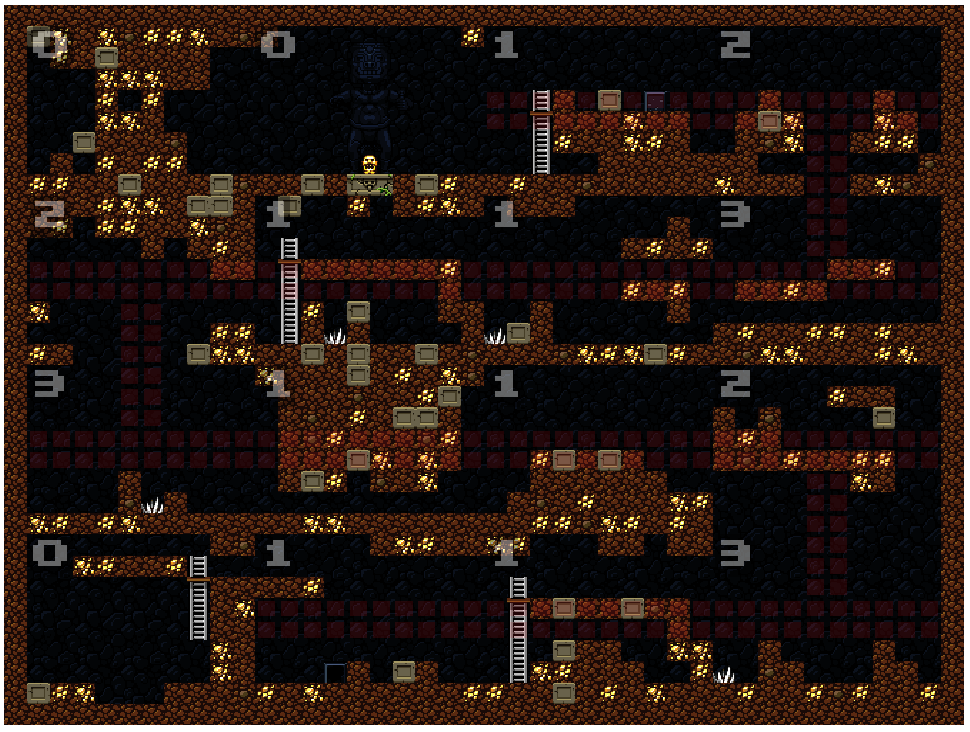
\includegraphics[width=.65\textwidth]{fig/spelunky-level-example.png}
\caption {\label{fig:spelunky-level-example}Exemplo de nível gerado
proceduralmente.} \end{figure}

Existe um grande número de ações -- e combinações de ações -- que podem ser
executadas pelo jogador a cada atualização do jogo. Algumas delas são
influenciadas por itens equipados ou estado atual do jogador, o que significa
que, caso não se tenha o devido cuidado, podem gerar resultados inesperados,
resultando na perda de vida ou até mesmo no fim do jogo. Os pontos de vida são o
recurso mais importante do explorador, pois quando esgotados, encerra-se a
partida. Existem inúmeras maneiras de se perder este recurso em Spelunky, como
inimigos, armadilhas ou até mesmo uma queda de um lugar muito alto.

A proposta desse trabalho é criar \textit{bots} capazes de se deslocar do início
ao fim de um nível de Spelunky, avaliando a qualidade destes através de métricas
tempo de jogo, número de vidas, entre outras.  Para auxiliar nesta tarefa,
utilizar-se-á o \textit{framework} SpelunkBots.  Esta ferramenta comunica-se
diretamente com o jogo, possibilitando a aquisição de informações do ambiente --
como localização de inimigos, armadilhas e tesouros --, o envio de ações para o
explorador, entre outras facilidades -- algumas mencionadas anteriormente.
